\cmfnewsection{Primeiros Passos no PSCAD}{./logos/fundo_tese}{0.15}





%%%%%%%%%%%%%%%%%%%%%%%%%%%%%%%%%%%%%%%%%%%%%%%%
%%%%%%%%%%%%%%%%%%%%%%%%%%%%%%%%%%%%%%%%%%%%%%%%
%%%%%%%%%%%%%%%%%%%%%%%%%%%%%%%%%%%%%%%%%%%%%%%%
%%%%%%%%%%%%%%%%%%%%%%%%%%%%%%%%%%%%%%%%%%%%%%%%
\begin{frame}{PSCAD: Versão Gratuita}
\centering

\begin{columns}
\column{0.3\linewidth}
apenas um teste

\column{0.7\linewidth}
\centering
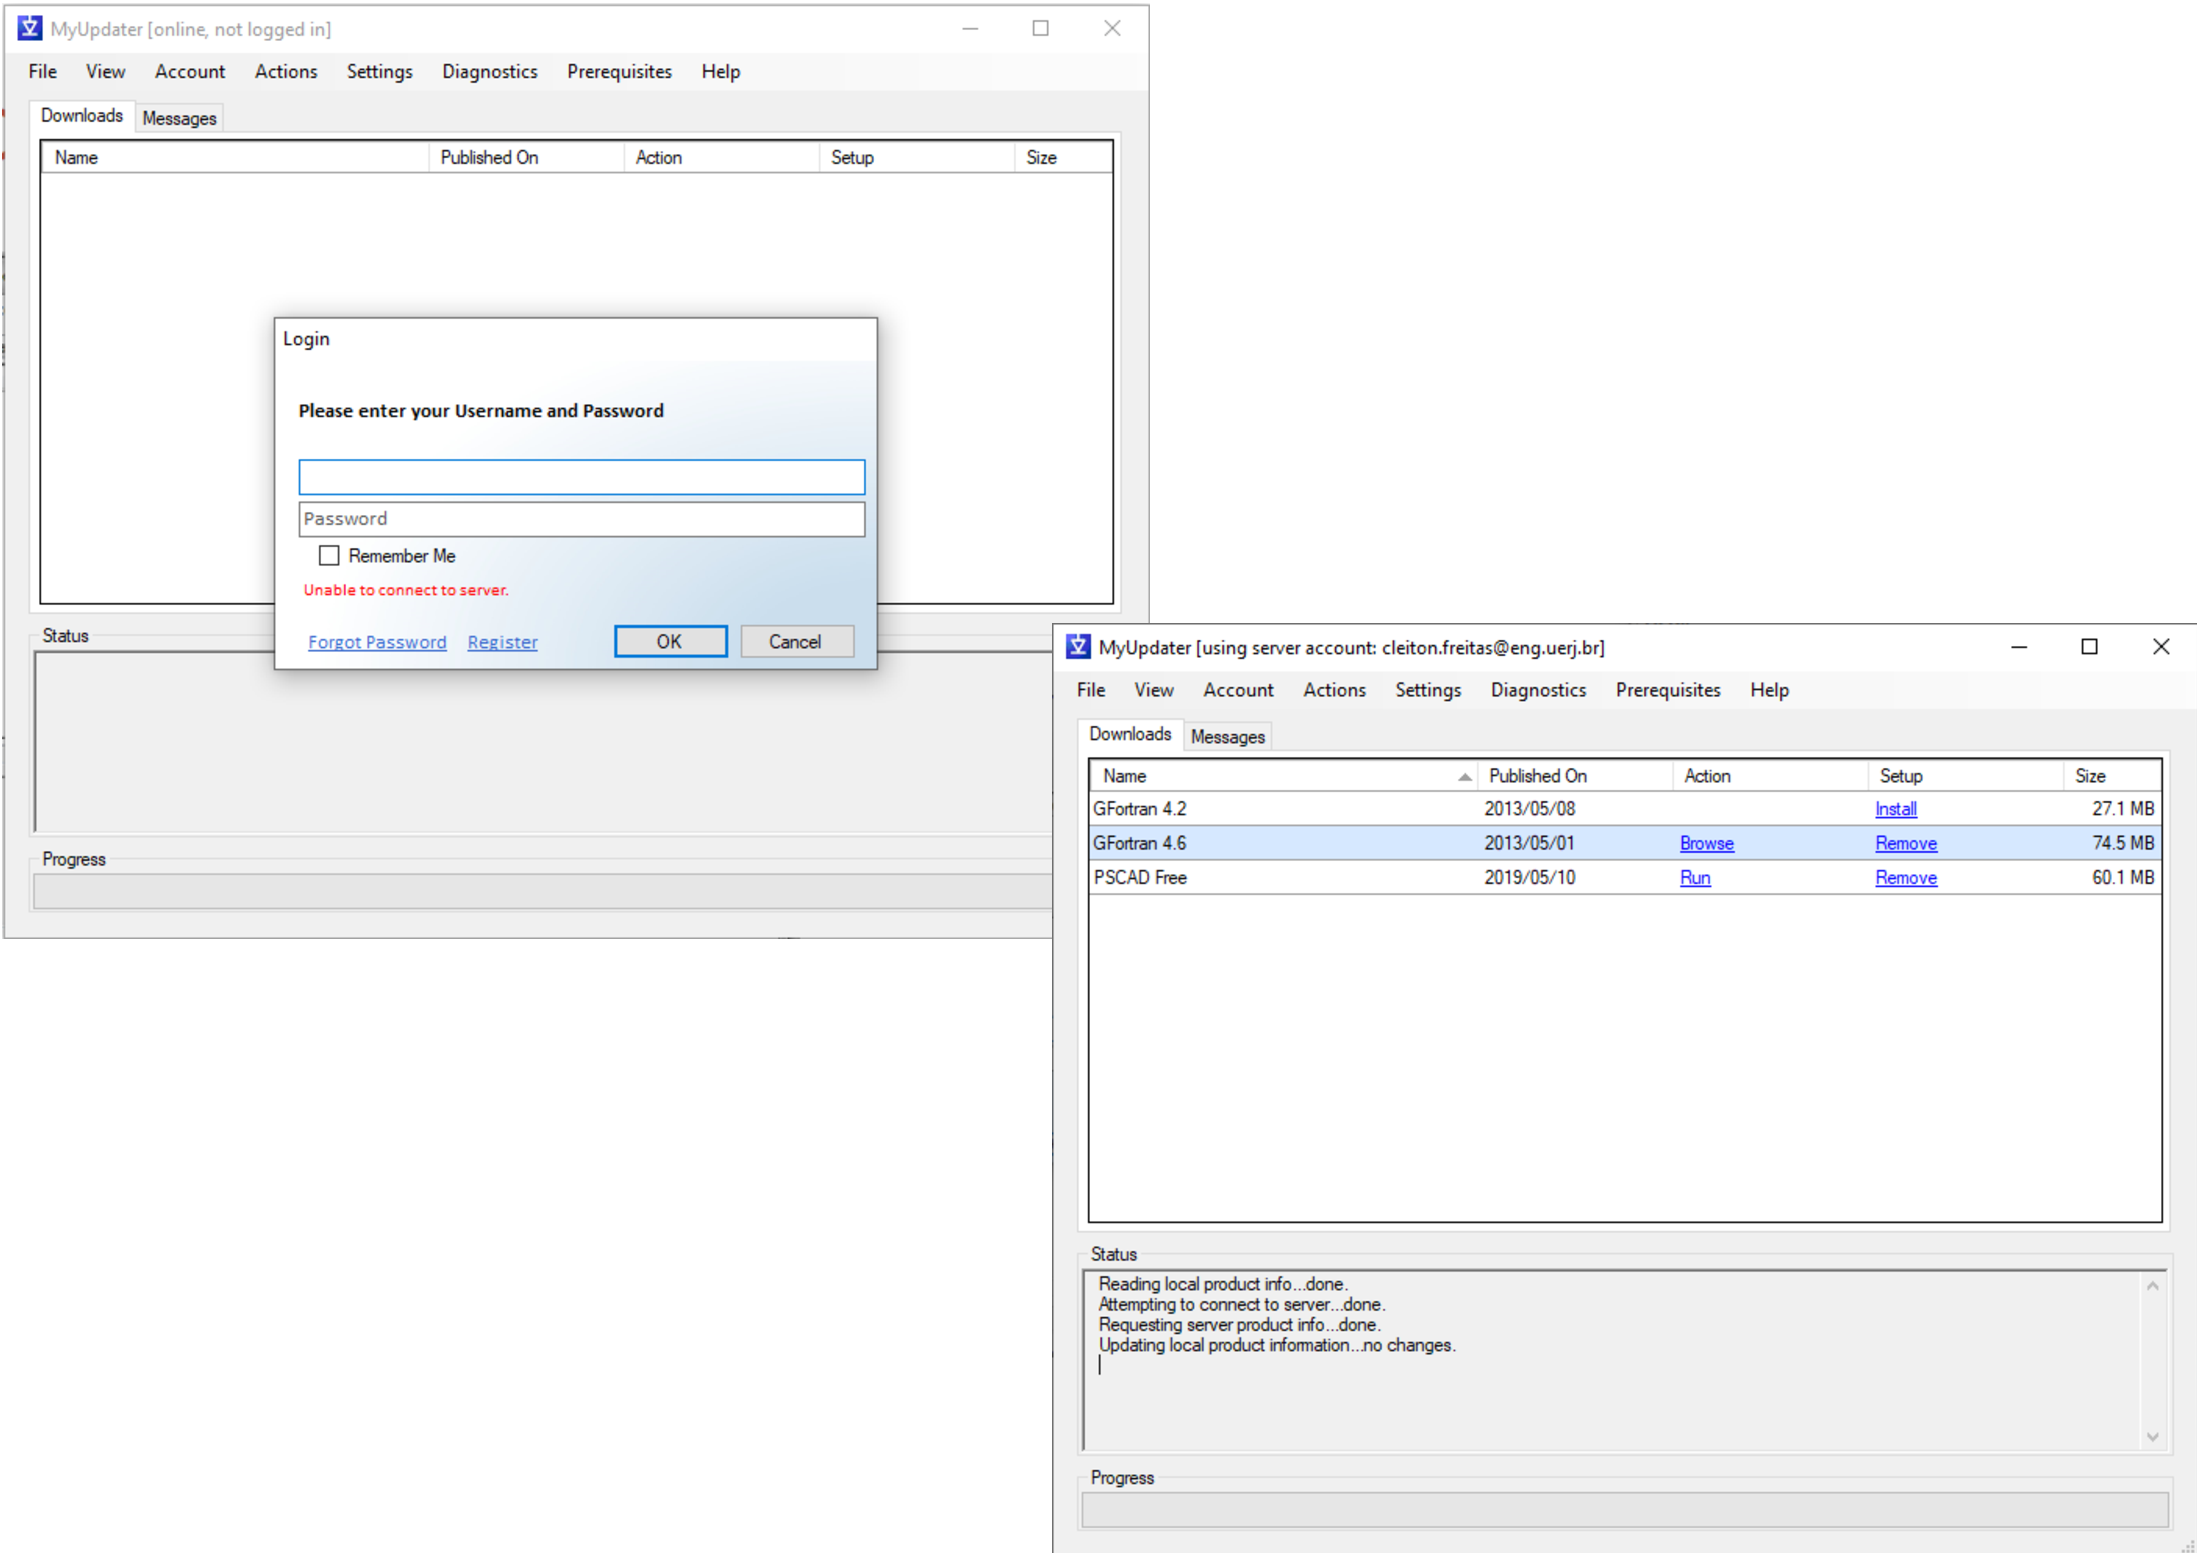
\includegraphics[width=0.8\linewidth]{./figuras/Primeiros-Passos/login}

\end{columns}

\end{frame}


%%%%%%%%%%%%%%%%%%%%%%%%%%%%%%%%%%%%%%%%%%%%%%%%
%%%%%%%%%%%%%%%%%%%%%%%%%%%%%%%%%%%%%%%%%%%%%%%%
%%%%%%%%%%%%%%%%%%%%%%%%%%%%%%%%%%%%%%%%%%%%%%%%
%%%%%%%%%%%%%%%%%%%%%%%%%%%%%%%%%%%%%%%%%%%%%%%%
\begin{frame}{PSCAD: Versão Gratuita}
\centering


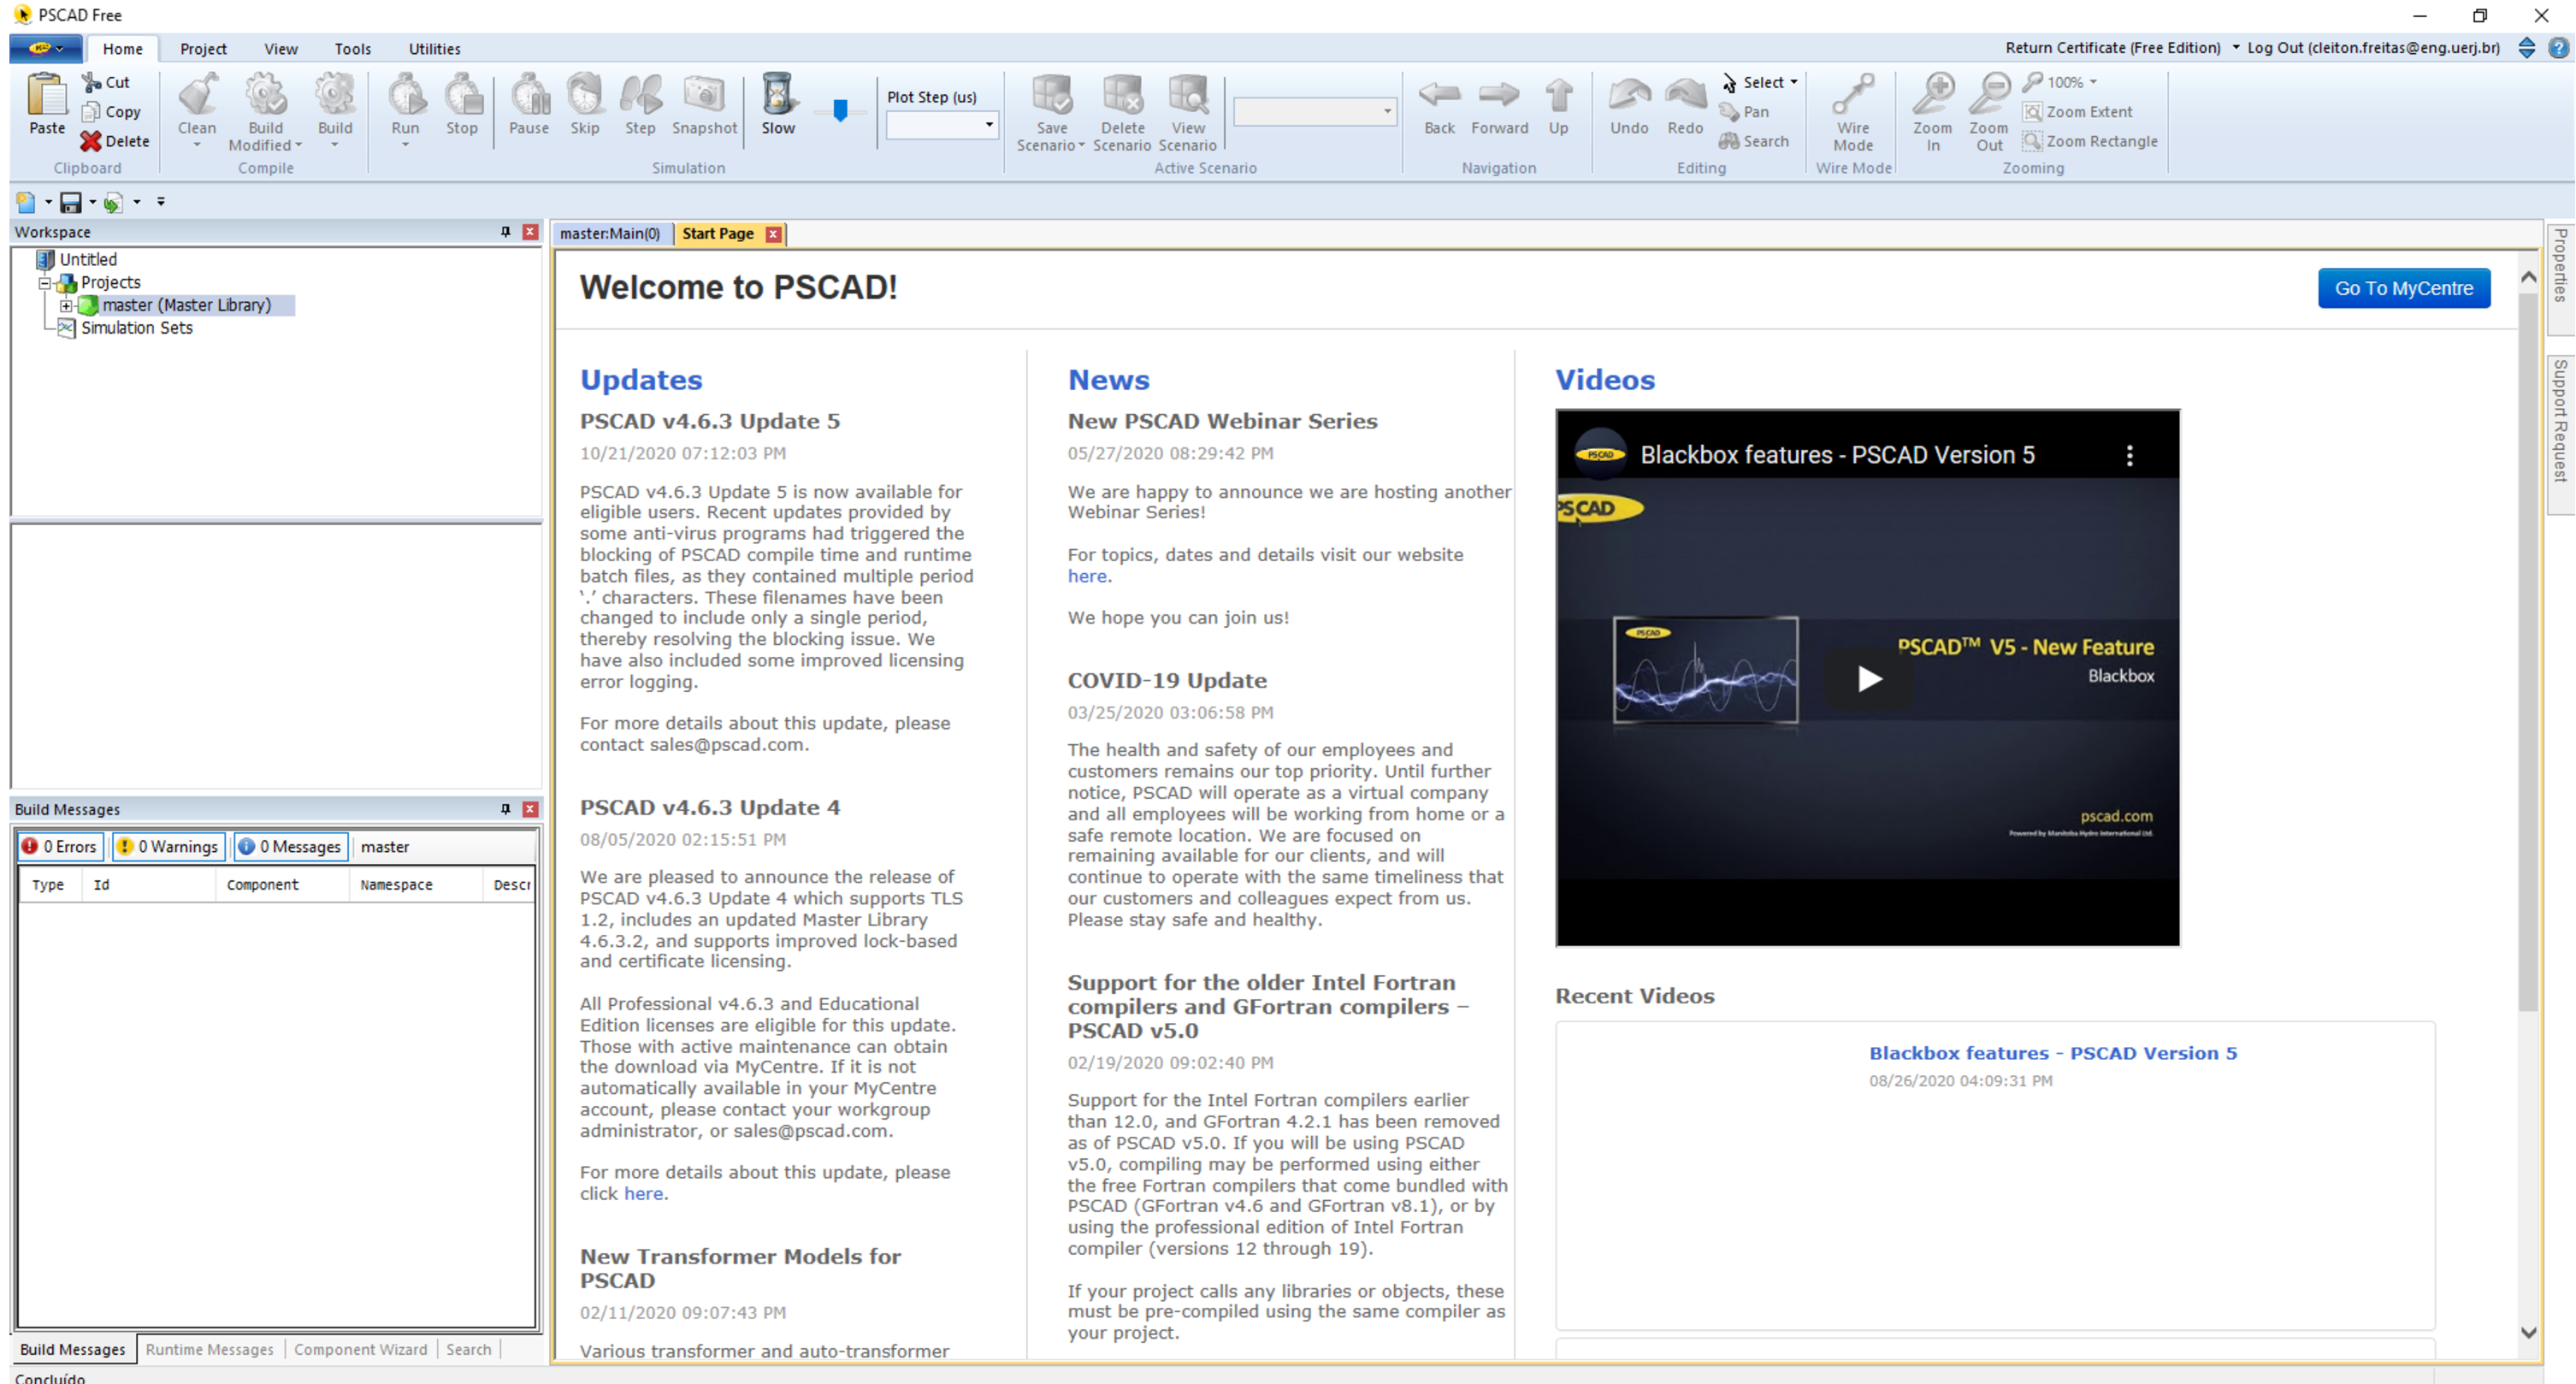
\includegraphics[width=0.85\linewidth]{./figuras/Primeiros-Passos/tela_inicial}


\end{frame}





%%%%%%%%%%%%%%%%%%%%%%%%%%%%%%%%%%%%%%%%%%%%%%%%
%%%%%%%%%%%%%%%%%%%%%%%%%%%%%%%%%%%%%%%%%%%%%%%%
%%%%%%%%%%%%%%%%%%%%%%%%%%%%%%%%%%%%%%%%%%%%%%%%
%%%%%%%%%%%%%%%%%%%%%%%%%%%%%%%%%%%%%%%%%%%%%%%%
\begin{frame}{PSCAD: Biblioteca Master}
\centering


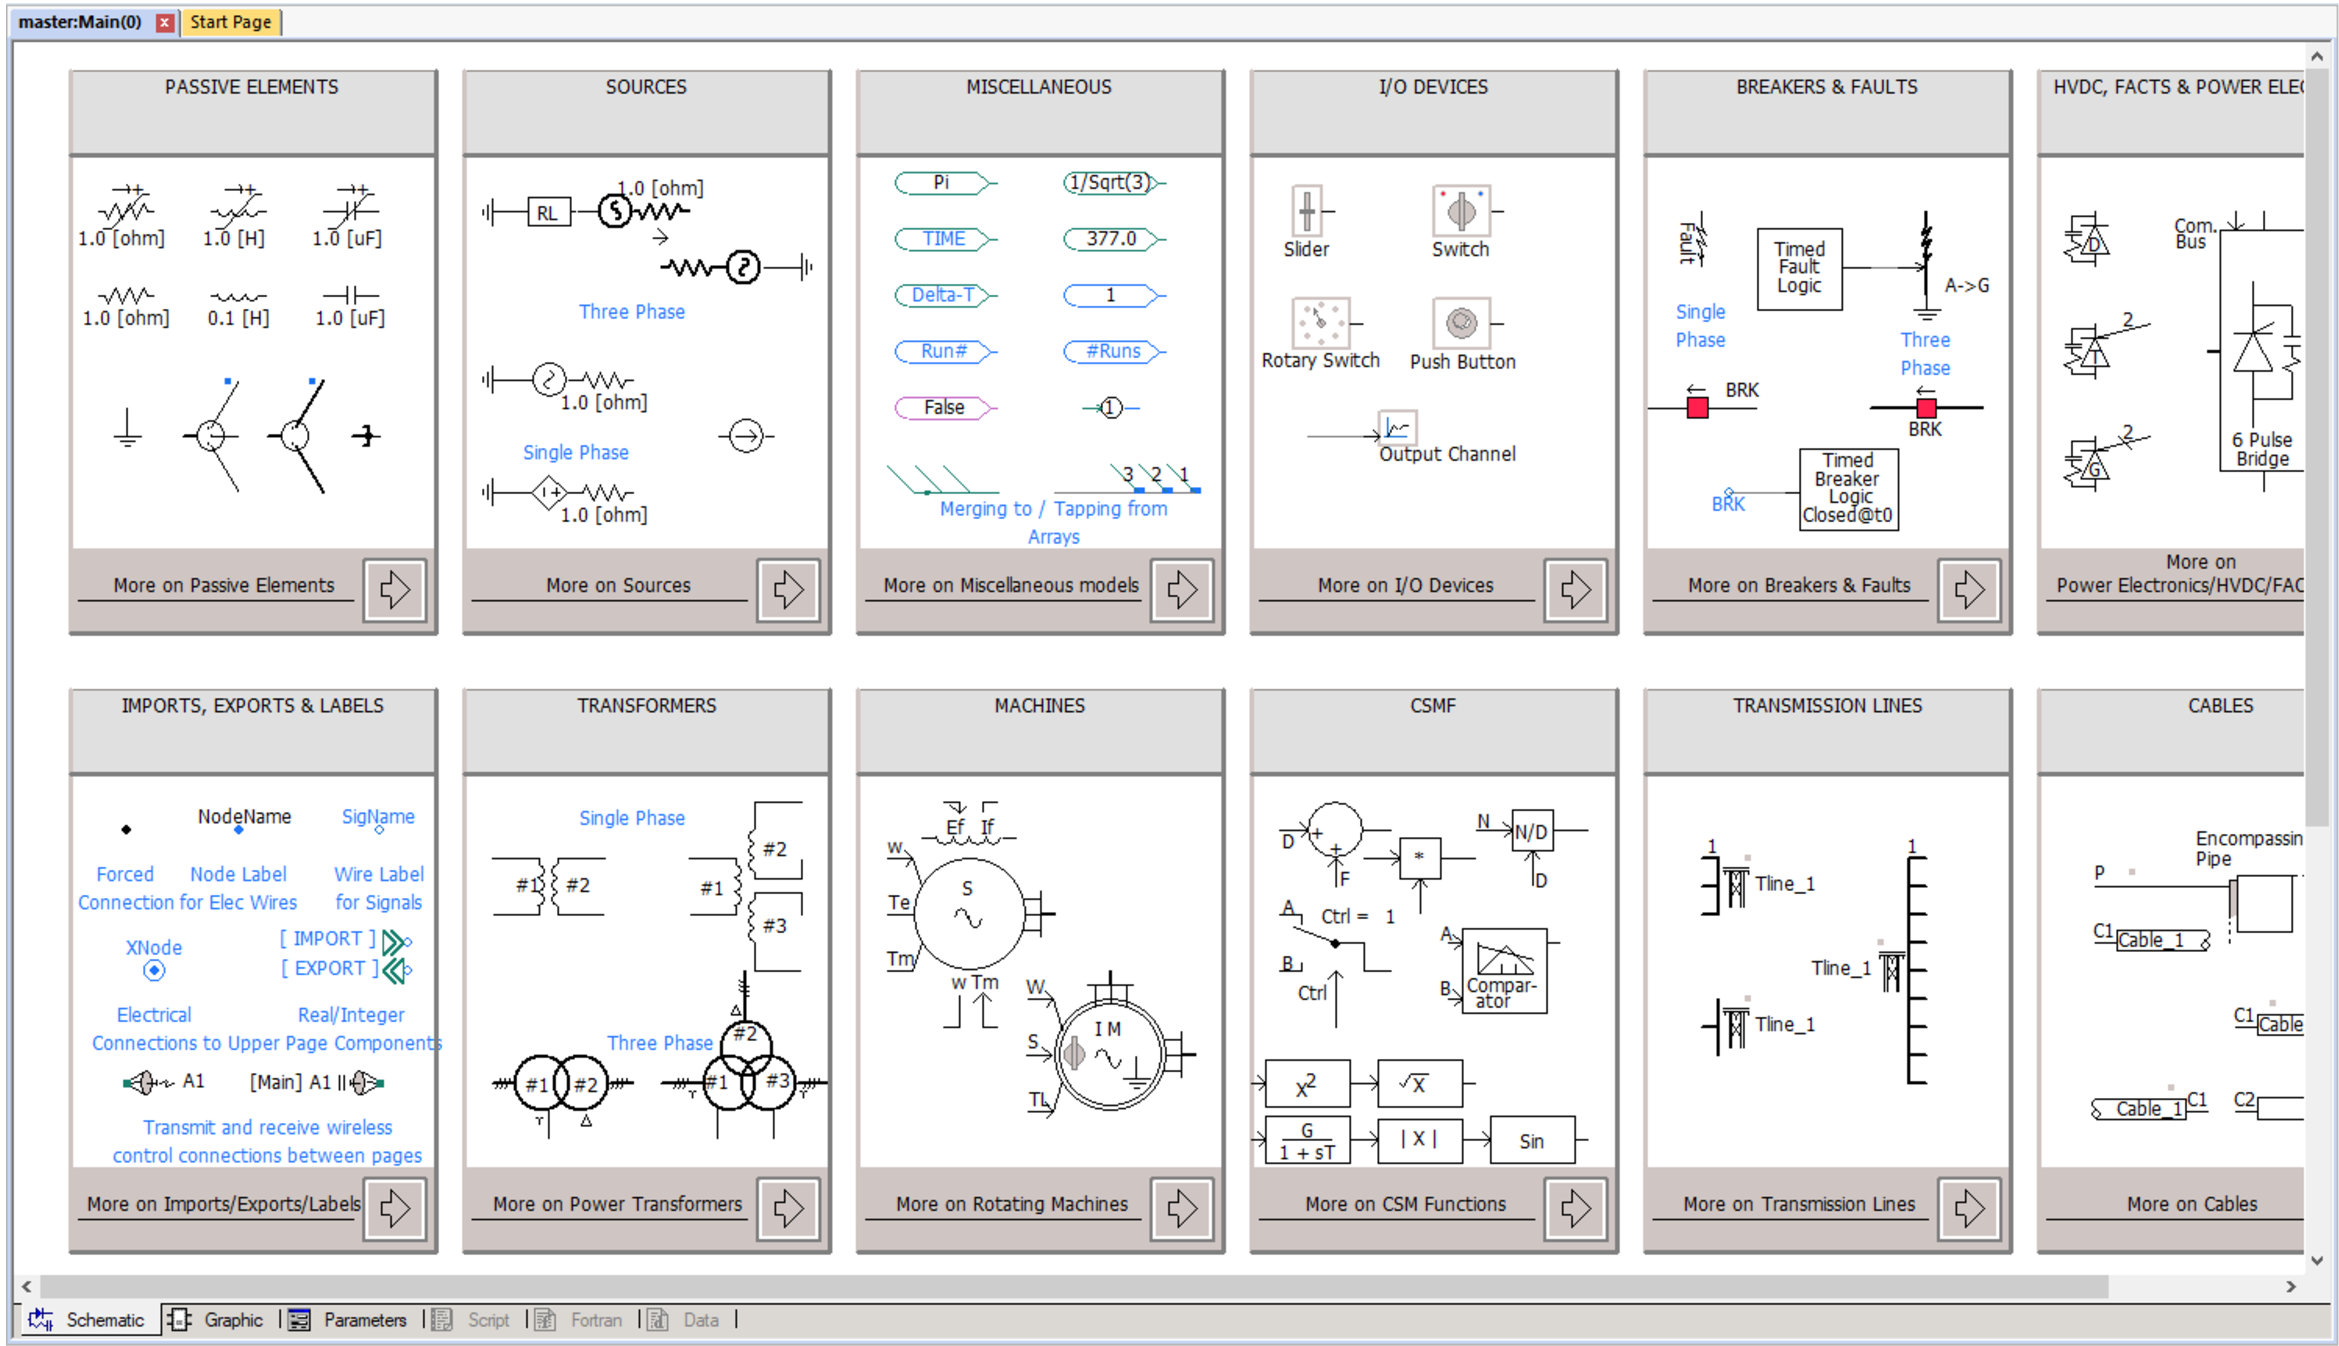
\includegraphics[width=0.85\linewidth]{./figuras/Primeiros-Passos/biblioteca_master}


\end{frame}




%%%%%%%%%%%%%%%%%%%%%%%%%%%%%%%%%%%%%%%%%%%%%%%%
%%%%%%%%%%%%%%%%%%%%%%%%%%%%%%%%%%%%%%%%%%%%%%%%
%%%%%%%%%%%%%%%%%%%%%%%%%%%%%%%%%%%%%%%%%%%%%%%%
%%%%%%%%%%%%%%%%%%%%%%%%%%%%%%%%%%%%%%%%%%%%%%%%
\begin{frame}{PSCAD: Biblioteca Master}
\centering


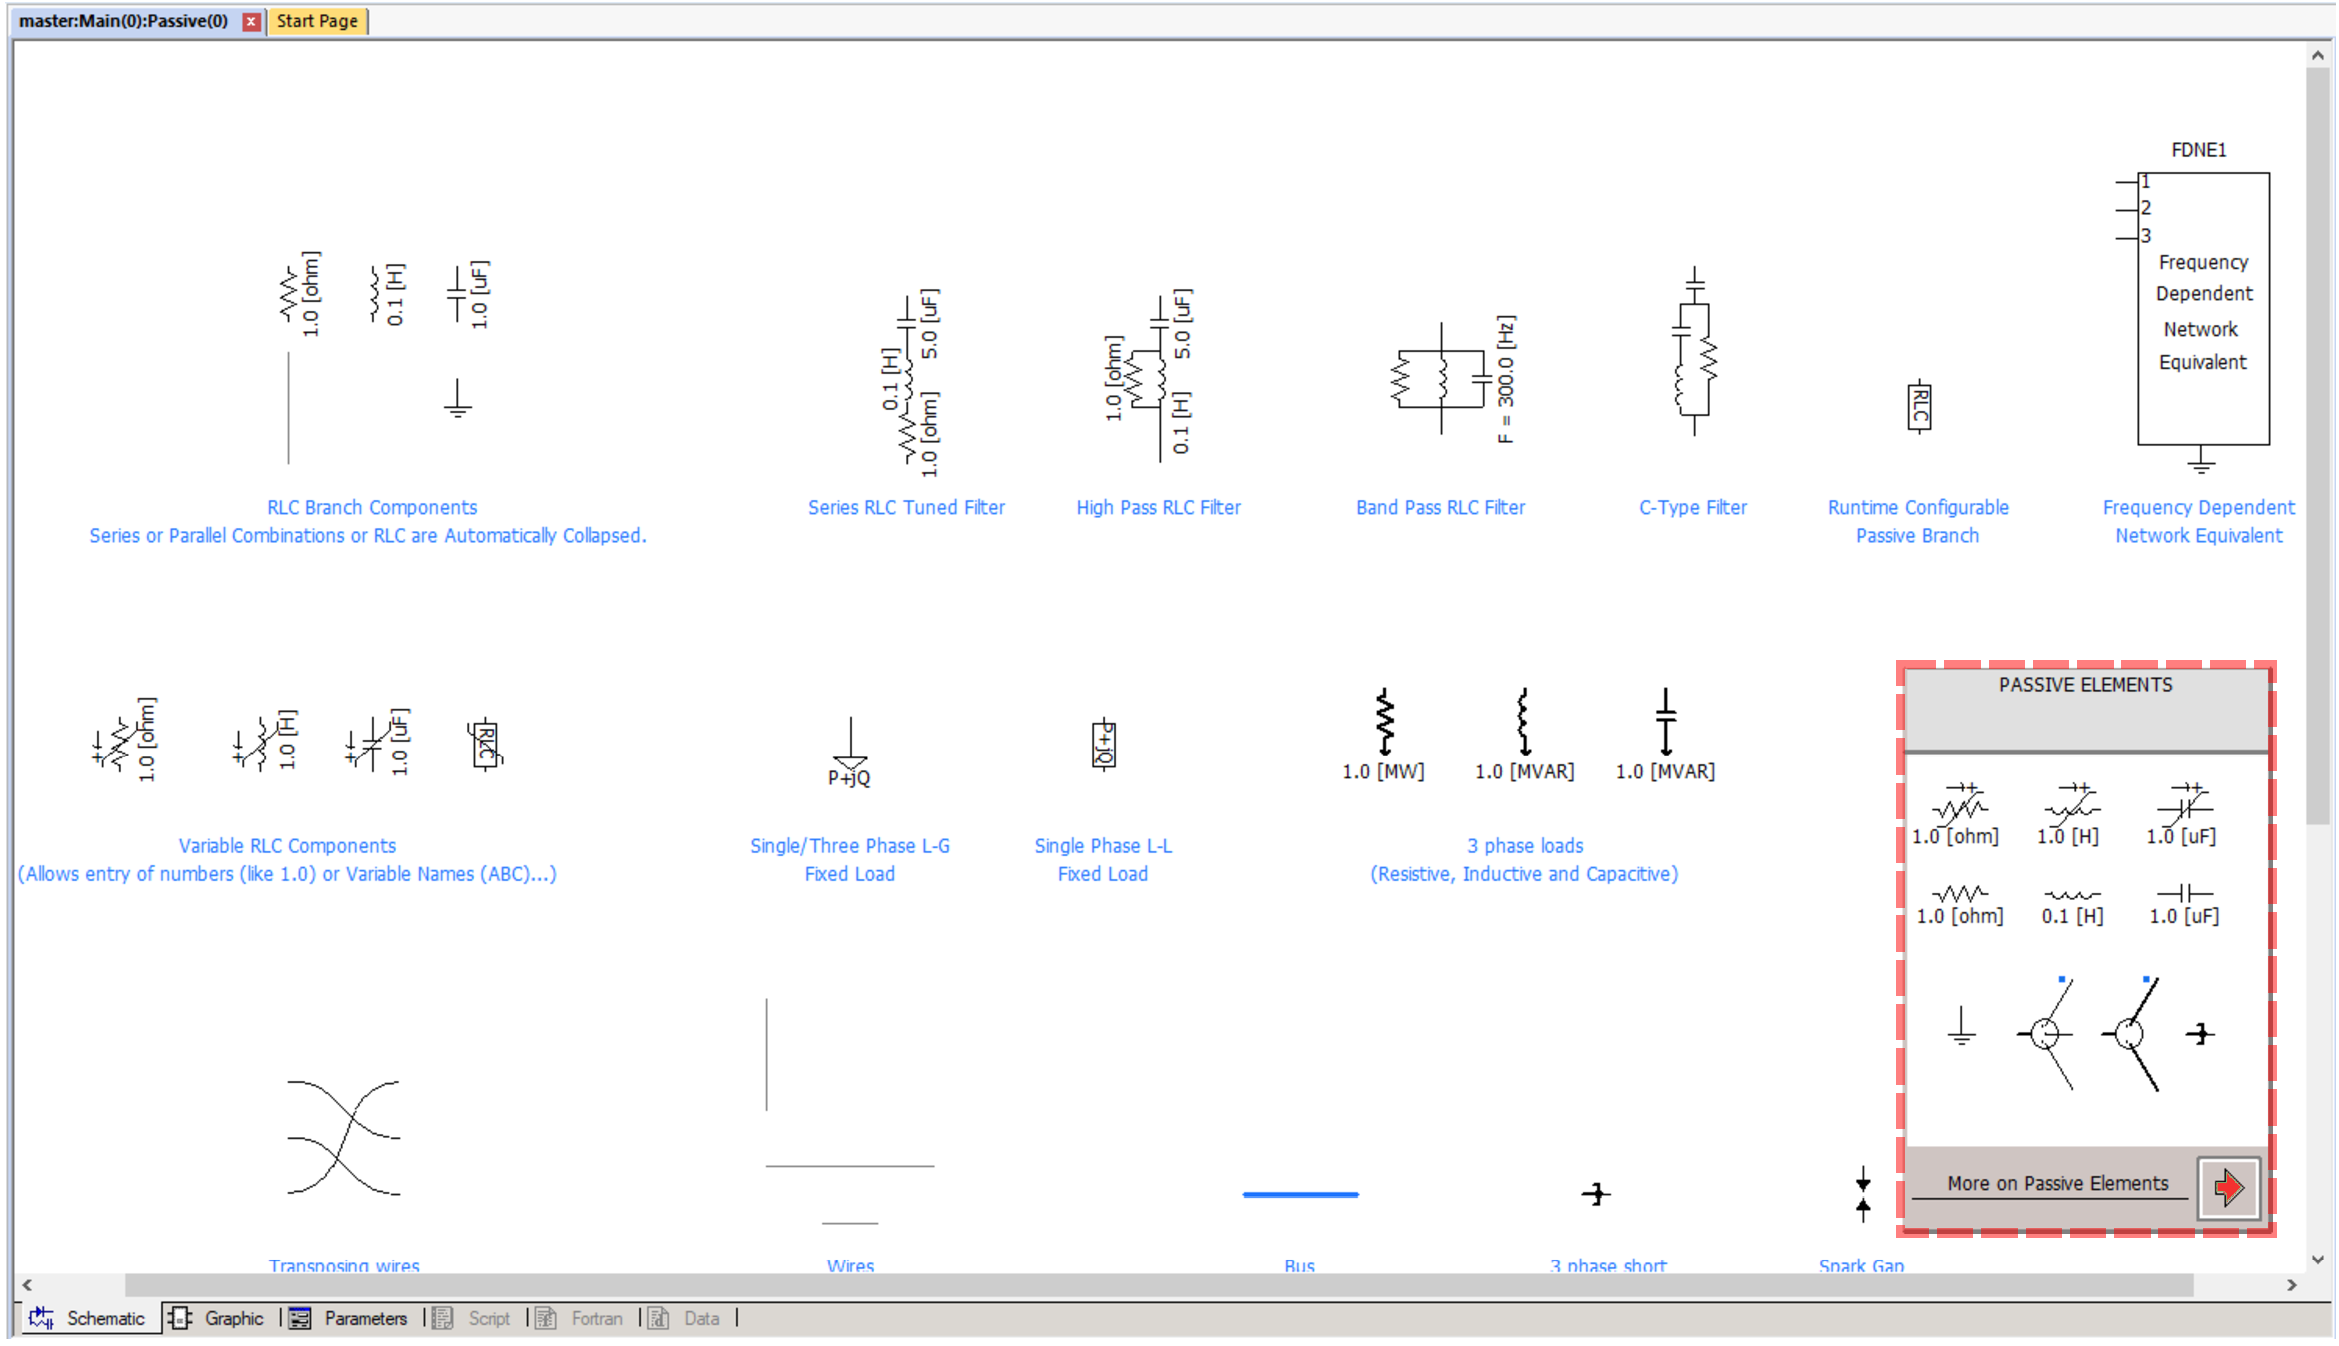
\includegraphics[width=0.85\linewidth]{./figuras/Primeiros-Passos/biblioteca_parte}


\end{frame}





%%%%%%%%%%%%%%%%%%%%%%%%%%%%%%%%%%%%%%%%%%%%%%%%
%%%%%%%%%%%%%%%%%%%%%%%%%%%%%%%%%%%%%%%%%%%%%%%%
%%%%%%%%%%%%%%%%%%%%%%%%%%%%%%%%%%%%%%%%%%%%%%%%
%%%%%%%%%%%%%%%%%%%%%%%%%%%%%%%%%%%%%%%%%%%%%%%%
\begin{frame}{PSCAD: Biblioteca Master}
\centering

Quando um projeto está aberto, também podemos acessar os componentes através dos seguintes menus.

\vspace*{1cm}

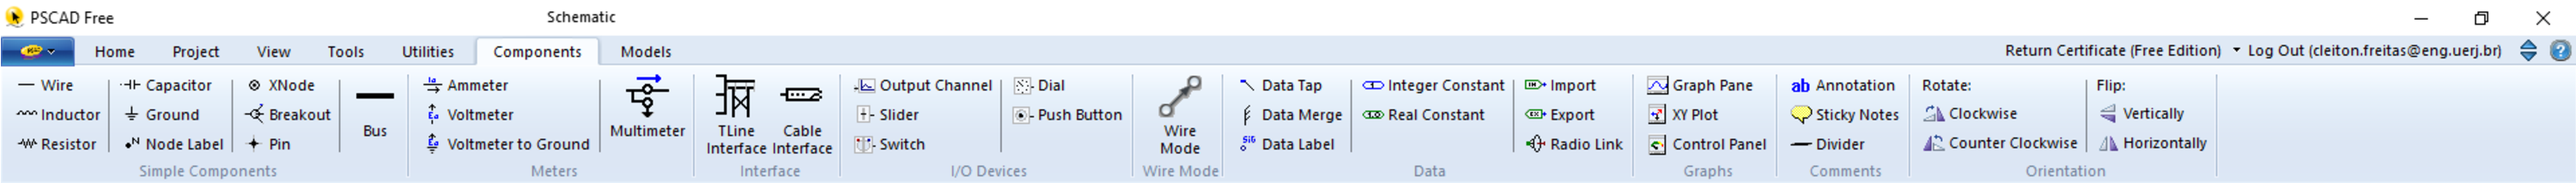
\includegraphics[width=0.85\linewidth]{./figuras/Primeiros-Passos/biblioteca_barra_components}
\vspace*{1cm}

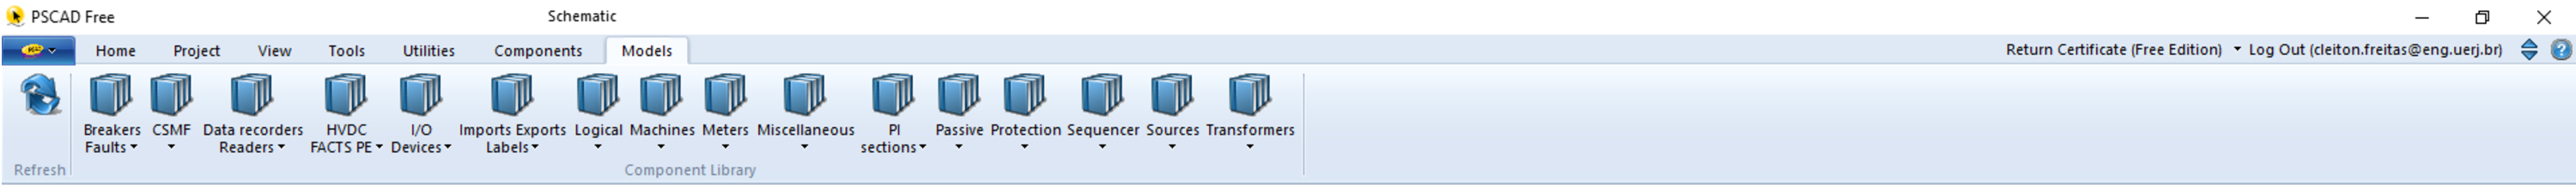
\includegraphics[width=0.85\linewidth]{./figuras/Primeiros-Passos/biblioteca_barra_models}

\end{frame}





%%%%%%%%%%%%%%%%%%%%%%%%%%%%%%%%%%%%%%%%%%%%%%%%
%%%%%%%%%%%%%%%%%%%%%%%%%%%%%%%%%%%%%%%%%%%%%%%%
%%%%%%%%%%%%%%%%%%%%%%%%%%%%%%%%%%%%%%%%%%%%%%%%
%%%%%%%%%%%%%%%%%%%%%%%%%%%%%%%%%%%%%%%%%%%%%%%%
\begin{frame}{Criando uma Simulação: {\it New Case}}
\centering


\begin{columns}


\column{0.5\linewidth}

\begin{itemize}
\item {\it New Case:} Cria uma nova simulação
\vspace*{1cm}
\item {\it Name:} Nome do arquivo de simulação
\vspace*{1cm}
\item {\it Path:} Lugar onde salvar a simulação
\end{itemize}
\vfill

\column{0.5\linewidth}

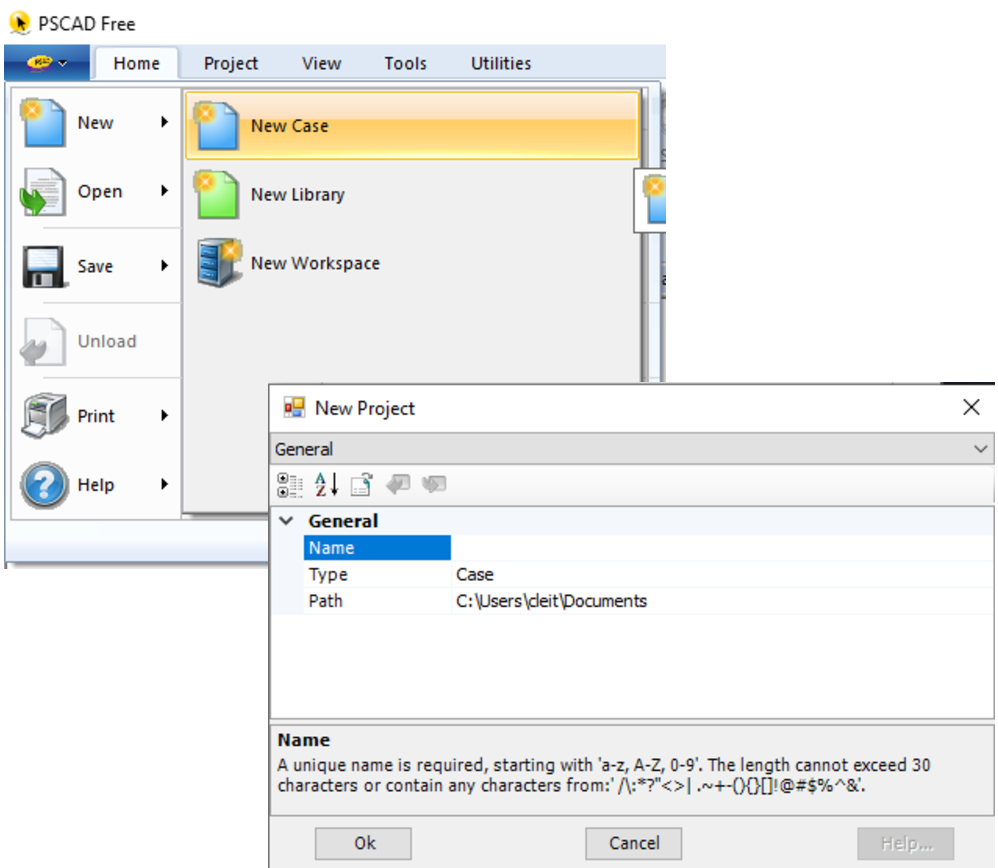
\includegraphics[width=0.95\linewidth]{./figuras/Primeiros-Passos/new_case}

\end{columns}




\end{frame}






%%%%%%%%%%%%%%%%%%%%%%%%%%%%%%%%%%%%%%%%%%%%%%%%
%%%%%%%%%%%%%%%%%%%%%%%%%%%%%%%%%%%%%%%%%%%%%%%%
%%%%%%%%%%%%%%%%%%%%%%%%%%%%%%%%%%%%%%%%%%%%%%%%
%%%%%%%%%%%%%%%%%%%%%%%%%%%%%%%%%%%%%%%%%%%%%%%%
\begin{frame}{Criando uma Simulação: Parâmetros do Projeto}
\centering

Menu {\it Project}

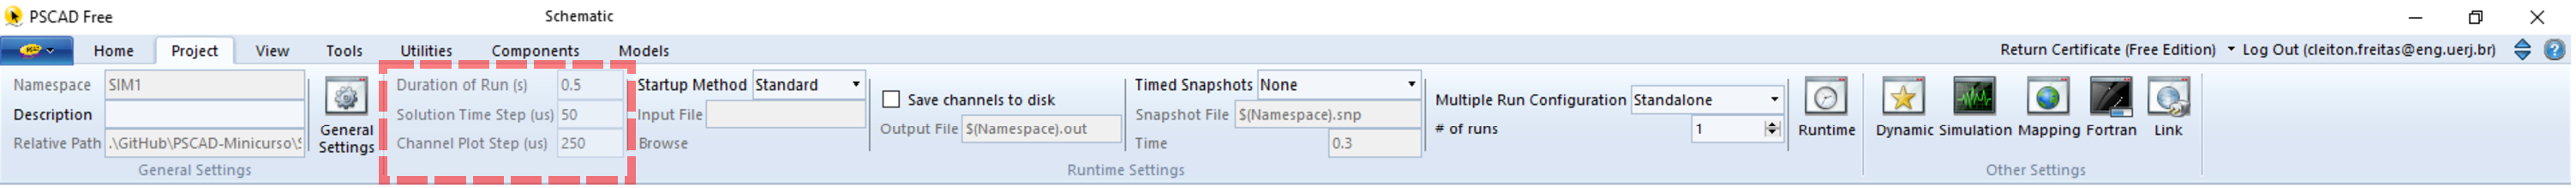
\includegraphics[width=0.95\linewidth]{./figuras/Primeiros-Passos/Project_parameters}


\begin{itemize}
\item {\it Duration of Run:} Tempo total de simulação
\vspace*{0.5cm}
\item {\it Time Step:} Intervalo de tempo entre os cálculos
\vspace*{0.5cm}
\item {\it Plot Step:} Intervalo de amostragem usado nos gráficos
\end{itemize}


\end{frame}





%%%%%%%%%%%%%%%%%%%%%%%%%%%%%%%%%%%%%%%%%%%%%%%%
%%%%%%%%%%%%%%%%%%%%%%%%%%%%%%%%%%%%%%%%%%%%%%%%
%%%%%%%%%%%%%%%%%%%%%%%%%%%%%%%%%%%%%%%%%%%%%%%%
%%%%%%%%%%%%%%%%%%%%%%%%%%%%%%%%%%%%%%%%%%%%%%%%
\begin{frame}{\color{blue} Importância do {Time Step}}
\centering
\color{blue}

\begin{columns}


\column{0.5\linewidth}
\centering
\textbf{Mundo Real:}

\begin{itemize}
\vspace*{0.5cm}
\item O mundo é contínuo
\vspace*{1cm}
\item Existe um número \textbf{INFINITO} de instantes em um intervalo de tempo  
\vspace*{1.5cm}
\end{itemize}




\column{0.5\linewidth}
\centering

\begin{equation*}
y(t) = \sin(120\pi t)
\end{equation*}

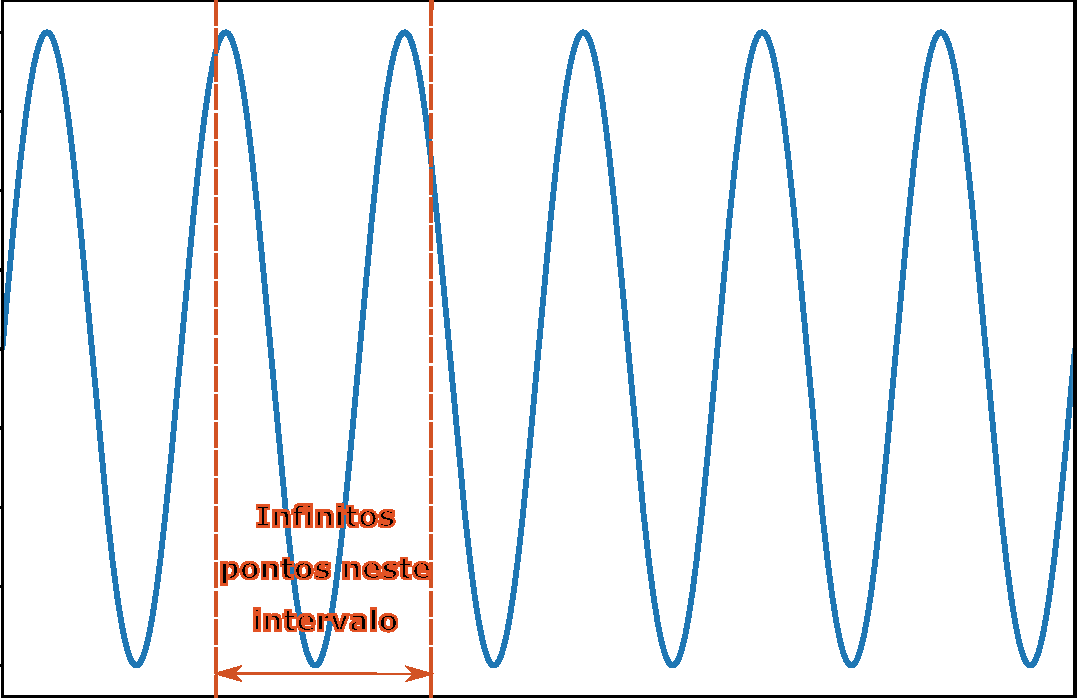
\includegraphics[width=0.95\linewidth]{./figuras/Primeiros-Passos/Sin_continuo}


\end{columns}



\end{frame}





%%%%%%%%%%%%%%%%%%%%%%%%%%%%%%%%%%%%%%%%%%%%%%%%
%%%%%%%%%%%%%%%%%%%%%%%%%%%%%%%%%%%%%%%%%%%%%%%%
%%%%%%%%%%%%%%%%%%%%%%%%%%%%%%%%%%%%%%%%%%%%%%%%
%%%%%%%%%%%%%%%%%%%%%%%%%%%%%%%%%%%%%%%%%%%%%%%%
\begin{frame}{\color{blue} Importância do {Time Step}}
\centering
\color{blue}

\begin{columns}


\column{0.5\linewidth}
\centering
\textbf{Simulação Digital:}

\begin{itemize}
\vspace{0.5cm}
\item O mundo é discreto
\vspace*{1cm}
\item Existe um número \textbf{FINITO} de instantes em um intervalo de tempo  
\end{itemize}

\column{0.5\linewidth}
\centering


\begin{equation*}
y[k T_s] = \sin(120\pi k T_s)
\end{equation*}
%


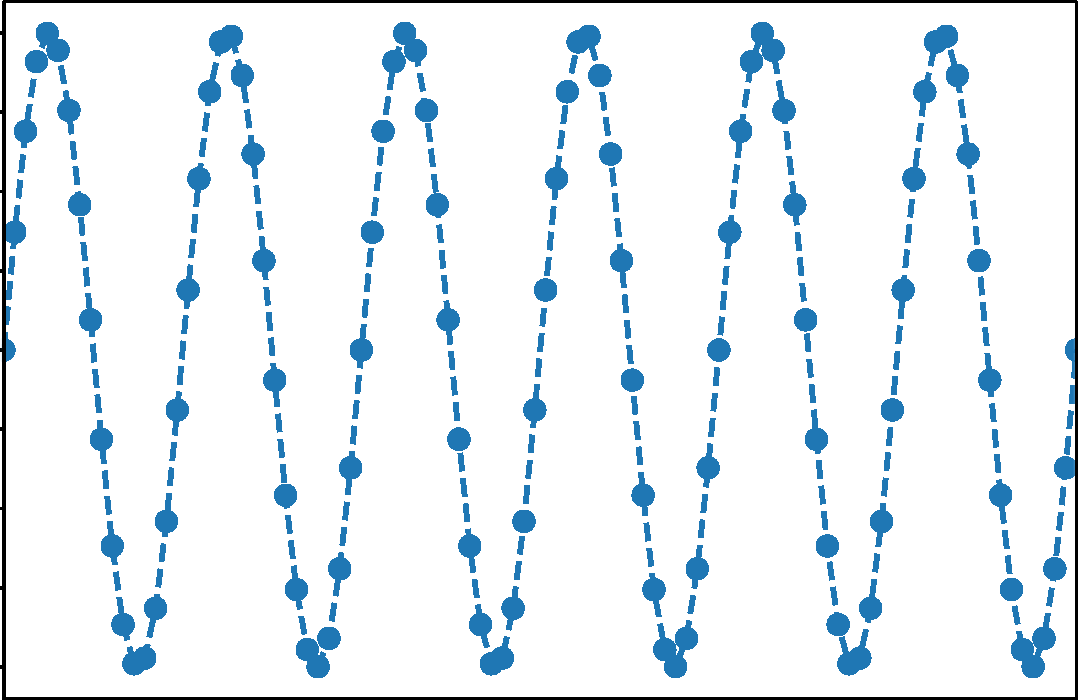
\includegraphics[width=0.95\linewidth]{./figuras/Primeiros-Passos/Sin_discreto1}


\end{columns}



\end{frame}







%%%%%%%%%%%%%%%%%%%%%%%%%%%%%%%%%%%%%%%%%%%%%%%%
%%%%%%%%%%%%%%%%%%%%%%%%%%%%%%%%%%%%%%%%%%%%%%%%
%%%%%%%%%%%%%%%%%%%%%%%%%%%%%%%%%%%%%%%%%%%%%%%%
%%%%%%%%%%%%%%%%%%%%%%%%%%%%%%%%%%%%%%%%%%%%%%%%
\begin{frame}{\color{blue} Importância do {Time Step}: ainda a senoide}
\centering
\color{blue}

\begin{columns}


\column{0.5\linewidth}
\centering
\textbf{Simulação Digital: Muito preciso}


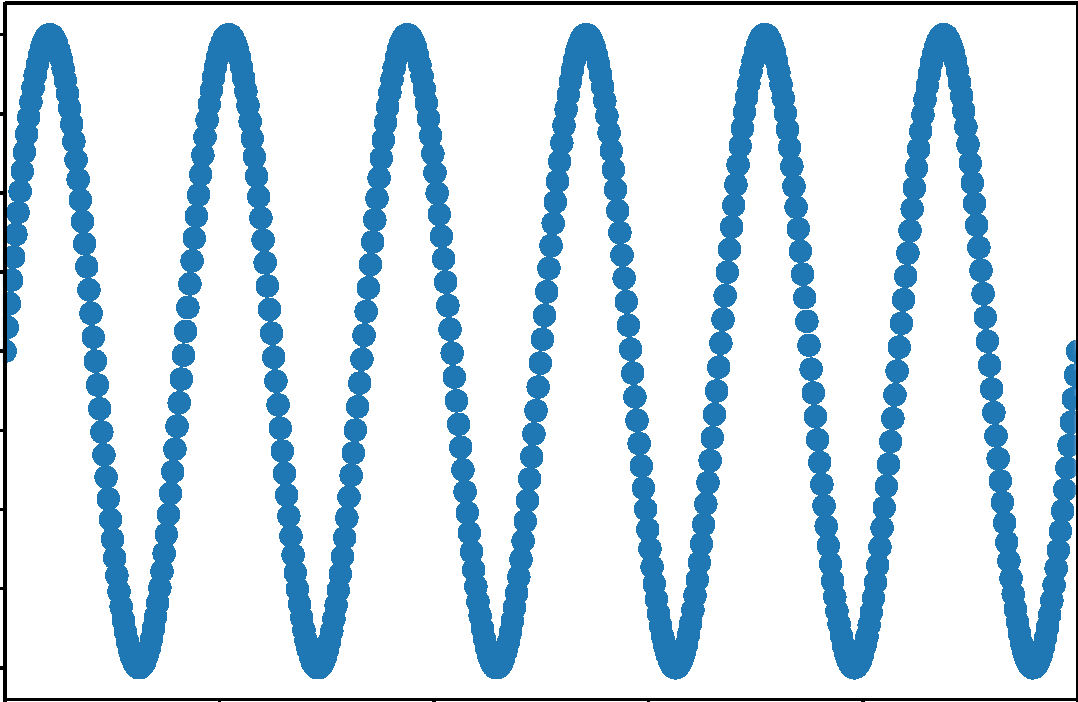
\includegraphics[width=0.95\linewidth]{./figuras/Primeiros-Passos/Sin_discreto1_muito}


\column{0.5\linewidth}
\centering
\textbf{Simulação Digital: Pouco preciso}


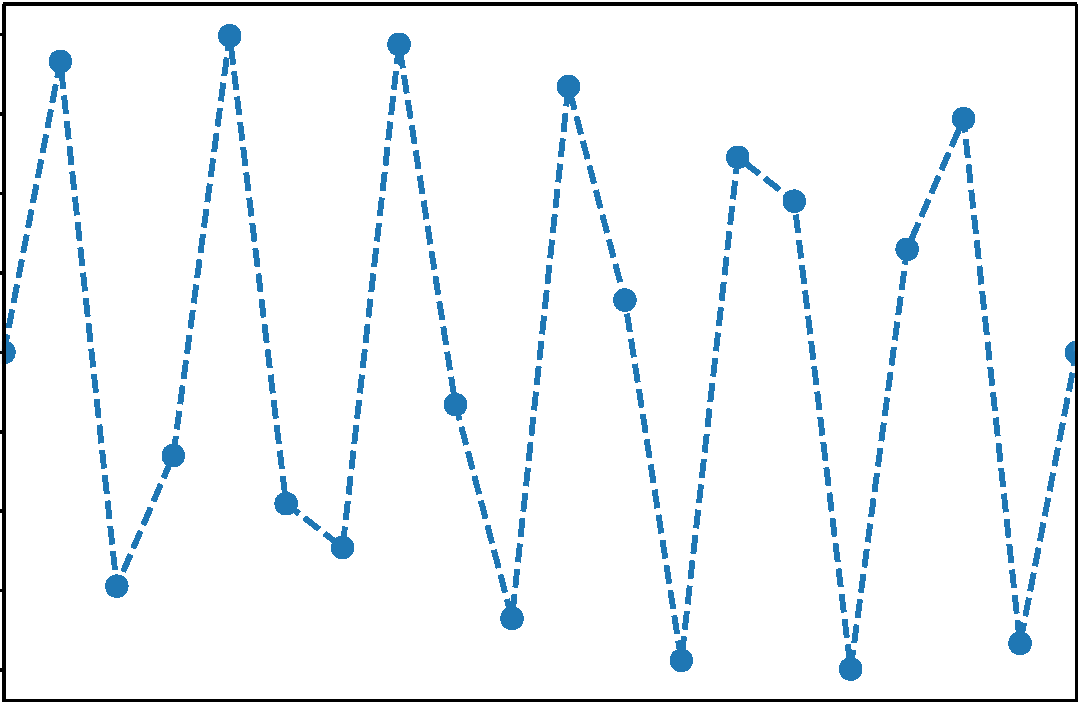
\includegraphics[width=0.95\linewidth]{./figuras/Primeiros-Passos/Sin_discreto1_pouco}


\end{columns}



\end{frame}







%%%%%%%%%%%%%%%%%%%%%%%%%%%%%%%%%%%%%%%%%%%%%%%%
%%%%%%%%%%%%%%%%%%%%%%%%%%%%%%%%%%%%%%%%%%%%%%%%
%%%%%%%%%%%%%%%%%%%%%%%%%%%%%%%%%%%%%%%%%%%%%%%%
%%%%%%%%%%%%%%%%%%%%%%%%%%%%%%%%%%%%%%%%%%%%%%%%
\begin{frame}{Criando uma Simulação: Continuando}
\centering


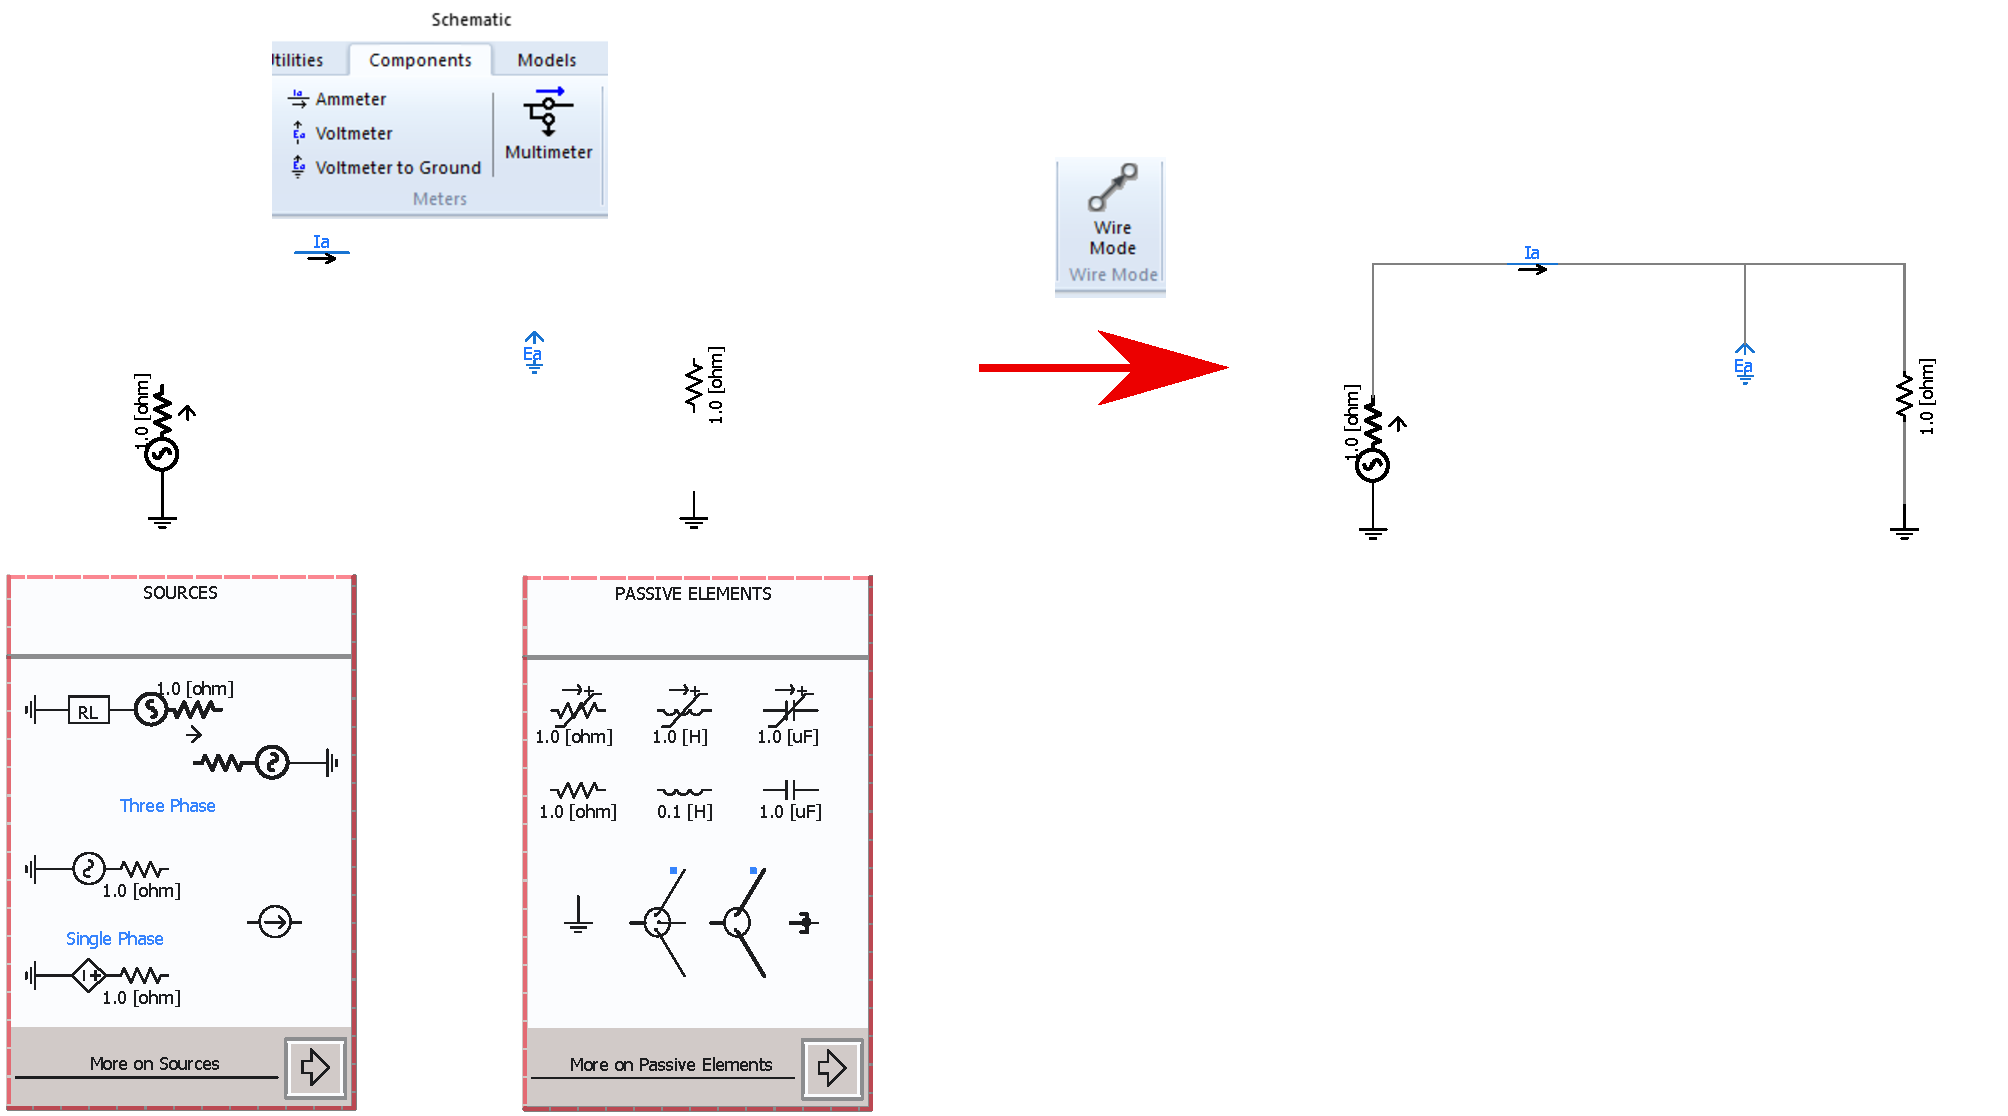
\includegraphics[width=0.85\linewidth]{./figuras/Primeiros-Passos/circuito1}



\end{frame}





%%%%%%%%%%%%%%%%%%%%%%%%%%%%%%%%%%%%%%%%%%%%%%%%
%%%%%%%%%%%%%%%%%%%%%%%%%%%%%%%%%%%%%%%%%%%%%%%%
%%%%%%%%%%%%%%%%%%%%%%%%%%%%%%%%%%%%%%%%%%%%%%%%
%%%%%%%%%%%%%%%%%%%%%%%%%%%%%%%%%%%%%%%%%%%%%%%%
\begin{frame}{Criando uma Simulação: Configuração dos componentes}
\centering


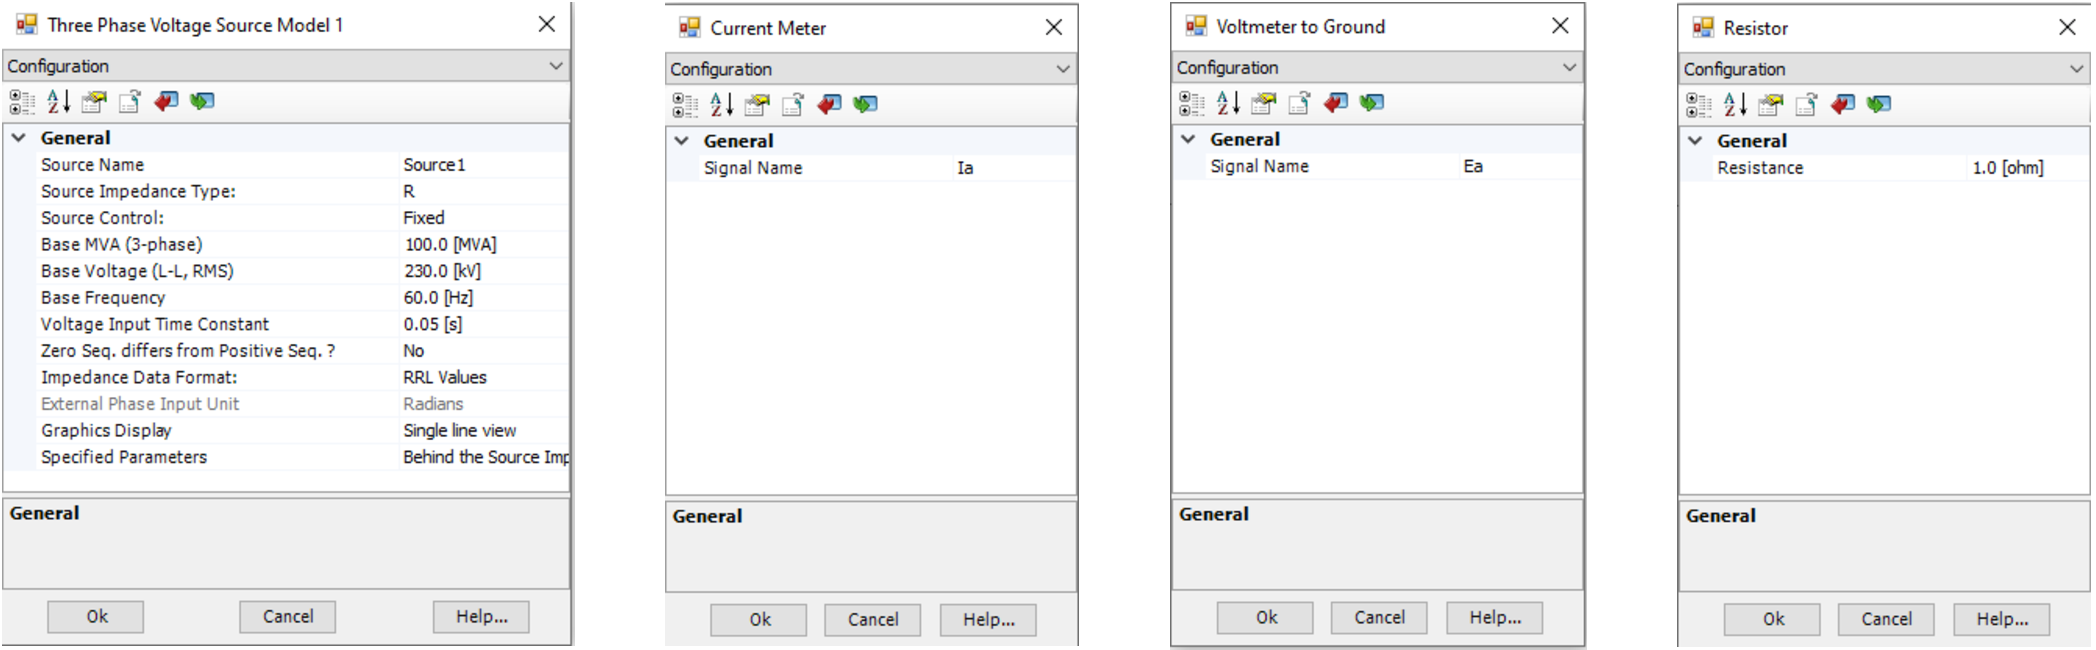
\includegraphics[width=0.85\linewidth]{./figuras/Primeiros-Passos/circuito1_Config_componentes}



\end{frame}




%%%%%%%%%%%%%%%%%%%%%%%%%%%%%%%%%%%%%%%%%%%%%%%%
%%%%%%%%%%%%%%%%%%%%%%%%%%%%%%%%%%%%%%%%%%%%%%%%
%%%%%%%%%%%%%%%%%%%%%%%%%%%%%%%%%%%%%%%%%%%%%%%%
%%%%%%%%%%%%%%%%%%%%%%%%%%%%%%%%%%%%%%%%%%%%%%%%
\begin{frame}{Criando uma Simulação: Gráficos}
\centering


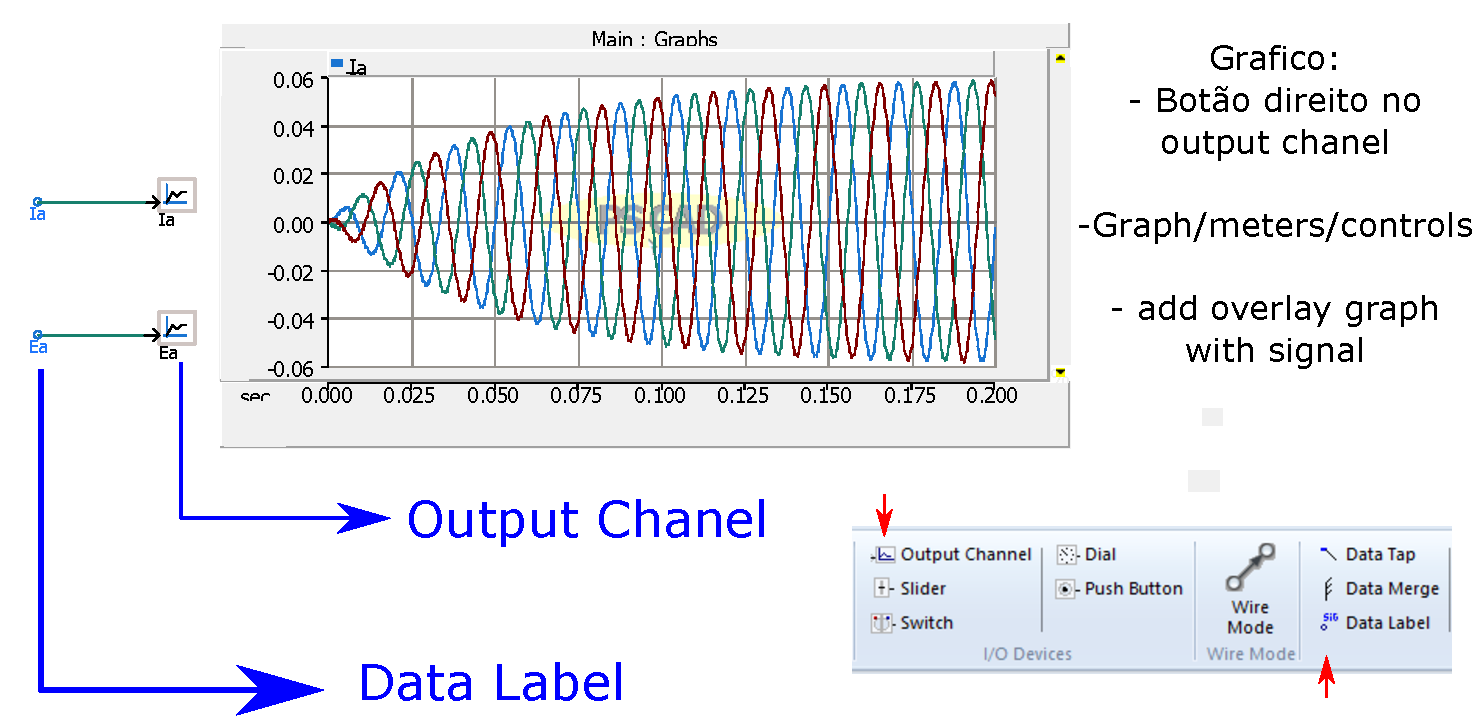
\includegraphics[width=0.85\linewidth]{./figuras/Primeiros-Passos/circuito1_grafico}



\end{frame}


